\begin{frame}{Timestamp Cyclical Encoding}
	\begin{columns}
		\column[c]{0.5\textwidth}
		%\footnotesize 
		We cyclically encoded timestamps using sine and cosine values to capture time patterns for minutes, hours, days, and years.
		\column[c]{0.5\textwidth}
		\begin{figure}
			\centering
			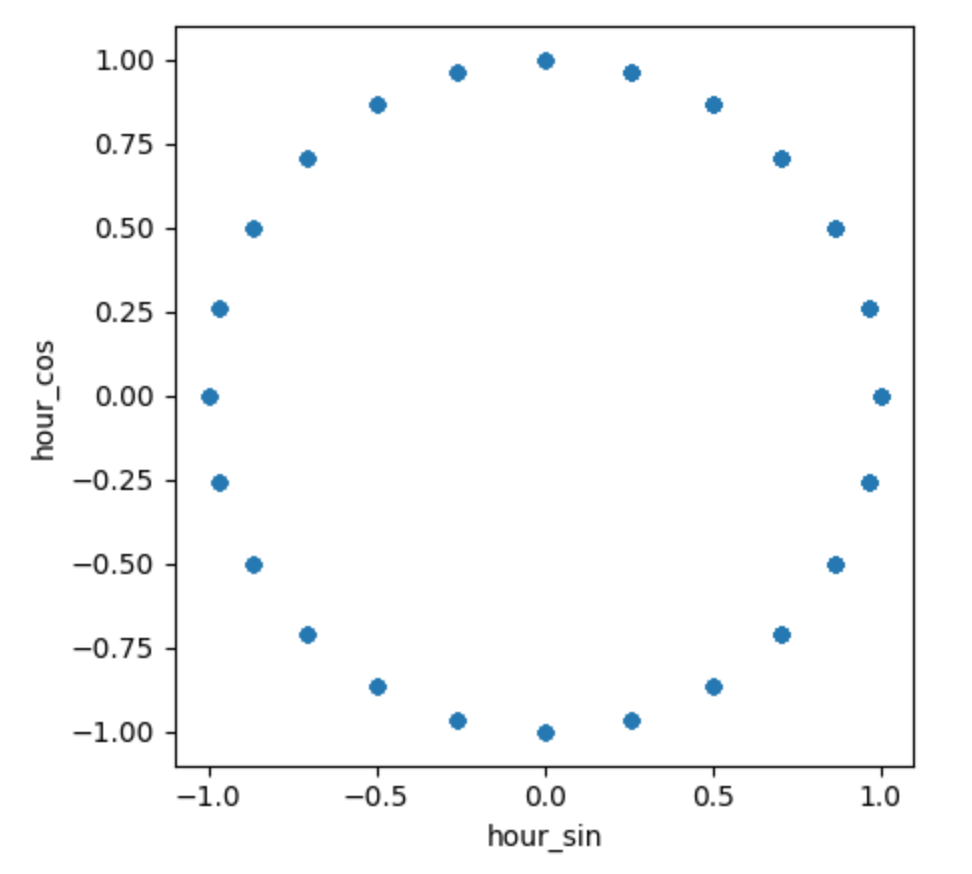
\includegraphics[width=\textwidth]{sections/2_preprocessing/imgs/tscyclic.png}
		\end{figure}
	\end{columns}
\end{frame}